\documentclass[manuscript,review,anonymous]{acmart}
\usepackage{tikz}
\usetikzlibrary{arrows.meta,positioning,fit}

\AtBeginDocument{%
  \providecommand\BibTeX{{Bib\TeX}}}

\setcopyright{none}
\settopmatter{printacmref=false}
\renewcommand\footnotetextcopyrightpermission[1]{}

\title{Beyond Human-Likeness: A Context-Aware Framework for Evaluating Appropriateness in Anthropomorphic AI Responses}

\author{Anonymous Author(s)}
\affiliation{%
  \institution{Anonymous Institution}
  \country{}}

\begin{abstract}
Human-like language is increasingly measurable in AI responses, but human-likeness alone does not determine whether anthropomorphic behavior is appropriate. A response can be warm and fluent while implying unsupported capacities such as feeling, memory, authority, or relationship; conversely, less human-like language can be more appropriate when it preserves boundaries and fits the situation. We present PERSONA, a context-aware evaluation framework that represents each response as a profile $P=(H,E,D,F)$: HuMT-derived human-likeness, empathic appropriateness, anthropomorphic deception/misleading implication risk, and contextual fit. PERSONA evaluates this profile against independently elicited overall anthropomorphic appropriateness ($OA$): five Group A raters scored $OA$, while five separate Group B raters scored $E$, $D$, and $F$. Across 1,490 responses in mental health, education, and health domains, grouped repeated cross-validation showed that $H$ alone was a weak and domain-dependent proxy for $OA$ (mental health $R^2=.026$, education $R^2=.099$, health $R^2=-.007$, pooled $R^2=.221$). The full profile improved prediction in mental health ($R^2=.659$), education ($R^2=.562$), and pooled analysis ($R^2=.499$); health was directionally positive ($R^2=.256$) but statistically uncertain because the gain's confidence interval crossed zero. The results support a calibration view: human-likeness is not wrong, but it is not enough.
\end{abstract}

\keywords{anthropomorphism, human-likeness, conversational AI, overall appropriateness, empathy, deception risk, contextual fit, evaluation}

\begin{document}
\maketitle

\section{Introduction}
Anthropomorphic language is now part of everyday interaction with generative AI systems. Assistants say ``I can help,'' offer reassurance, explain uncertainty, apologize, encourage, and sometimes imply care, memory, personal experience, or expertise. These linguistic choices matter because they shape how people understand what an AI system is, what it can do, and what kind of relationship is being enacted in the interaction.

Recent work has made human-likeness itself more measurable. HumT provides an automated measure of human-like tone in LLM outputs \cite{Cheng2025HumT}; DeVrio et al. provide a taxonomy of linguistic expressions that contribute to anthropomorphism in language technologies \cite{DeVrio2025Taxonomy}; and prior work documents personification cues and their potential harms in dialogue systems \cite{Abercrombie2023Mirages}. This is an important foundation. However, the central HCI challenge is not simply measuring how human-like an AI response appears, but determining when anthropomorphic behavior is appropriate.

Our answer is not that human-likeness is incorrect or should be minimized. Human-like language can make systems more understandable, supportive, and usable. The problem is that human-likeness is a descriptive signal, not an appropriateness criterion. It does not by itself say whether warmth was calibrated, whether a response implied capacities the system does not possess, or whether the response matched the user's situation. In a crisis prompt, appropriateness may require urgent safety guidance rather than elaborate reassurance. In an educational prompt, approachable language may help, but false intimacy or overconfident authority may still be inappropriate. In a health prompt, uncertainty and referral boundaries can matter more than a conversational style.

We introduce PERSONA, a framework for evaluating contextual appropriateness in anthropomorphic AI responses. PERSONA represents each response as a profile:
\[
P = (H, E, D, F)
\]
where $H$ is human-likeness, $E$ is empathic appropriateness, $D$ is anthropomorphic deception/misleading implication risk, and $F$ is contextual fit. The framework is intentionally multidimensional. It treats human-likeness as one useful signal while separating it from empathy, misleading implication risk, and contextual fit.

The empirical design addresses a major weakness of our earlier formulation: circularity. Overall appropriateness ($OA$) is not computed from the same dimensions used to predict it. Instead, we collect holistic $OA$ judgments from one rater group and $E$, $D$, and $F$ judgments from a separate rater group. This makes the relationship between the profile and appropriateness an empirical question rather than a scoring identity.

We evaluate PERSONA on 1,490 AI responses across three domains: mental health ($n=660$), education ($n=415$), and health ($n=415$). The mental health domain is the primary empirical setting because it has the strongest prompt structure and full coverage. Education provides strong cross-domain evidence, while health is interpreted cautiously because overall appropriateness is ceiling-heavy. We ask whether human-likeness alone predicts overall anthropomorphic appropriateness, whether the full profile adds information beyond human-likeness, and how associations between dimensions and appropriateness vary across domains.

This paper contributes:
\begin{itemize}
  \item a context-aware construct model for anthropomorphic AI evaluation that distinguishes human-likeness, empathic appropriateness, deception risk, and contextual fit;
  \item an annotation design that separates holistic appropriateness judgments from predictor-dimension judgments;
  \item a multi-domain dataset and reproducible analysis pipeline for evaluating the relationship between anthropomorphic signals and appropriateness;
  \item empirical evidence that human-likeness alone is a weak and domain-dependent proxy for overall anthropomorphic appropriateness, especially compared with the full profile in mental health and education contexts.
\end{itemize}

The practical motivation is straightforward. If an evaluation system only asks whether a response is human-like, it cannot distinguish at least four cases that matter for design: appropriately warm support, excessive intimacy, misleading claims of human capacity, and contextually wrong but fluent advice. These cases may look similar under a single human-likeness score. PERSONA is designed to make them separable.

\section{Related Work}
\subsection{Anthropomorphism as Linguistic Signalling}
Anthropomorphism is often understood as the attribution of human-like qualities to non-human entities \cite{Epley2007Anthropomorphism}. In AI systems, this attribution is shaped by both user-side factors and system-side cues. People differ in their tendency to anthropomorphize \cite{Waytz2010WhoSeesHuman}, and motivational conditions can make human-like interpretation more likely \cite{Epley2008NeedHuman}. At the same time, system outputs supply concrete cues that invite or discourage such interpretation.

The HCI literature has long shown that people respond socially to computers and media technologies when systems present social cues \cite{Nass1994CASA,Reeves1996MediaEquation,NassMoon2000Mindlessness}. Relational-agent work then explored how systems can be designed to build and maintain longer-term social-emotional relationships with users \cite{Bickmore2005RelationalAgents}. Conversational-agent research further taxonomizes social cues and shows how anthropomorphic design, identity, and conversational signals affect perceptions of humanness and social presence \cite{Feine2019SocialCues,Araujo2018ChatbotHype,GoSundar2019Humanizing}. This tradition motivates PERSONA's concern: social language is not merely decorative interface style; it changes the relationship users may infer.

For text-based systems, those cues are linguistic. DeVrio et al.'s taxonomy is especially important for PERSONA because it gives a vocabulary for the textual properties through which language technologies become anthropomorphic \cite{DeVrio2025Taxonomy}. Rather than treating anthropomorphism as a single impression, the taxonomy foregrounds different kinds of expressions that can carry human-like implications. PERSONA builds on this insight but asks a different question: once anthropomorphic cues are present, are they appropriate in the context?

HumT operationalizes one part of this space by measuring human-like language in LLM outputs \cite{Cheng2025HumT}. This makes $H$ scalable and independent from human ratings. However, HumT measures textual human-likeness, not whether a response is appropriate, truthful about system capacities, or fitted to the user's needs. PERSONA therefore uses HumT as one profile dimension rather than as the target variable.

\subsection{Empathy, Deception, and Fit}
Empathy in text-based support can be decomposed into distinguishable communicative mechanisms, including emotional reactions, interpretations, and explorations \cite{Sharma2020Empathy}. PERSONA adopts the view that empathy is linguistically observable, but changes the evaluation target from amount of empathy to appropriateness of empathy. A response can contain empathic language while still being mismatched, generic, excessive, or action-displacing.

Recent systems can already produce responses that are rated as highly empathic in health-adjacent settings \cite{Ayers2023PhysicianChatbot}, and computational work has attempted to improve empathic conversational behavior \cite{Sharma2021EmpathyRL}. These findings make empathy evaluation urgent, but they also show why measuring empathy quantity is not enough. PERSONA's $E$ asks whether empathic language is calibrated to the prompt rather than whether the response simply contains more emotional support.

Deception risk captures a different problem. Work on honest and dishonest anthropomorphism argues that human-like cues can mislead users when they imply capacities or relationships a system does not actually have \cite{Kaminski2017RobotEyes,Leong2019Dishonest}. Social robotics has similarly treated deception as a design problem even when no human designer intends to deceive in a narrow psychological sense \cite{Sharkey2021Deception}. PERSONA operationalizes this as $D$: the degree to which the response implies human experience, feeling, memory, identity, authority, continuity, or dependency. This is connected to, but not identical with, human-likeness. A response can be conversational without being deceptive, and a formal response can still make misleading claims of authority.

Contextual fit captures whether the response is the right kind of response for the user's situation. This construct is necessary because appropriateness is not a generic quality judgment. The same tone, certainty, or level of detail can be suitable in one setting and unsuitable in another. Contextual integrity theory makes this broader point in privacy: what is appropriate depends on context-specific norms rather than universal information rules \cite{Nissenbaum2004ContextualIntegrity}. PERSONA applies the same context-relative logic to conversational response behavior.

\subsection{From Human-Likeness to Contextual Appropriateness}
The central claim is a calibration claim. Human-likeness can be valuable, but its value depends on what the interaction calls for and what the language implies. Existing work motivates this shift: anthropomorphic cues have varied forms \cite{DeVrio2025Taxonomy}, measurable surface properties \cite{Cheng2025HumT}, and potential transparency and reliance risks \cite{Abercrombie2023Mirages,Leong2019Dishonest}. PERSONA contributes a measurement framework that puts these channels into one empirical profile and tests them against independent appropriateness judgments.

This distinction is also important for regulation and governance. Disclosure requirements, such as those in the European Union's AI Act, address whether people are informed that they are interacting with an AI system \cite{EUAIAct2024}. Disclosure is necessary, but it is not the same as turn-level appropriateness. A system can disclose that it is an AI and still repeatedly imply personal feeling, memory, authority, or relationship through its wording. PERSONA is not a legal compliance tool, but it provides a way to measure the response-level linguistic behaviors that make these concerns concrete.

This problem also sits within broader concerns about language-model risks, over-reliance, and anthropomorphic framing. Taxonomies of language-model risks identify unsafe use, manipulation, and deception as human-computer interaction harms \cite{Weidinger2022Risks}. Trust in automation research argues that good design should support appropriate reliance rather than overtrust or undertrust \cite{LeeSee2004Trust}, and HCI work shows that interaction designs can reduce overreliance on AI advice \cite{Bucinca2021CognitiveForcing}. Recent discussions of LLMs also warn that imprecise language about systems knowing, believing, or feeling can invite anthropomorphic misunderstanding \cite{Shanahan2024Talking}, while critiques of AI discourse emphasize the social cost of blurring machine behavior with human cognition \cite{Bender2024Dehumanization}.

Historically, these concerns are not new. ELIZA already demonstrated that simple language patterns could invite people to treat a program as a meaningful conversational partner \cite{Weizenbaum1966ELIZA}. Later work on social and relational technologies warned that people may expect more from machines as they become socially expressive \cite{Turkle2011AloneTogether}. PERSONA updates this long-standing issue for contemporary LLM responses by measuring the linguistic profile of anthropomorphic behavior and testing it against independently elicited appropriateness.

\section{The PERSONA Framework}
\subsection{Constructs}
PERSONA defines four response-level dimensions.

\textbf{$H$: Human-likeness.} $H$ is the degree to which the response exhibits linguistic features conventionally associated with human speakers, such as conversational register, first-person framing, personal stance, and informal discourse cues. In this study, $H$ is measured automatically with HumT \cite{Cheng2025HumT}. $H$ is descriptive, not evaluative.

\textbf{$E$: Empathic appropriateness.} $E$ is the degree to which the response provides calibrated warmth, emotional recognition, and validation that are useful for the user's situation. It is not simply the amount of empathy. A factual education prompt may require little emotional language; a mental health prompt may require affective recognition but not excessive intimacy.

\textbf{$D$: Anthropomorphic deception/misleading implication risk.} $D$ is the risk that anthropomorphic behavior creates misleading implications about the system's capabilities, internal states, relationships, experiences, or authority. It is not intentional deception by the AI. Examples include claims of feeling, memory, personal care, permanent commitment, exclusivity, or professional authority. Functional first-person language alone is not treated as deception risk.

\textbf{$F$: Contextual fit.} $F$ is the degree to which the response's content, action, tone, certainty, and role boundaries match the primary situation. It is not generic response quality. It asks whether this is the right response posture for this prompt.

\subsection{Using DeVrio et al.'s Taxonomy}
DeVrio et al.'s taxonomy helps ground PERSONA at the linguistic level \cite{DeVrio2025Taxonomy}. It shows that anthropomorphism is not a vague overall feeling but is produced through identifiable textual expressions. PERSONA uses that insight in three ways.

First, $E$ focuses on the empathic subset of linguistic behavior: emotional recognition, validation, and support. These expressions may increase human-likeness, but PERSONA asks whether they are calibrated to the situation. Second, $D$ focuses on expressions whose human-like implications can become misleading: claims of feeling, personal experience, memory, authority, relationship, or dependency. Third, $F$ evaluates whether the same linguistic posture fits the interactional context. A taxonomy of anthropomorphic expressions tells us what kinds of cues are present; PERSONA asks how those cues function in context.

\subsection{Overall Appropriateness as an Independent Criterion}
The target variable, $OA$, is a holistic judgment of whether the response is appropriate overall. PERSONA does not define $OA$ as a weighted sum of $H$, $E$, $D$, and $F$. Instead, $OA$ is collected separately. This is the methodological difference that allows the framework to be tested. If $OA$ were derived from the profile, high predictive performance would be circular; because $OA$ is independently elicited, predictive performance estimates whether the profile captures information that human raters treat as relevant to appropriateness.

\begin{figure}
  \centering
  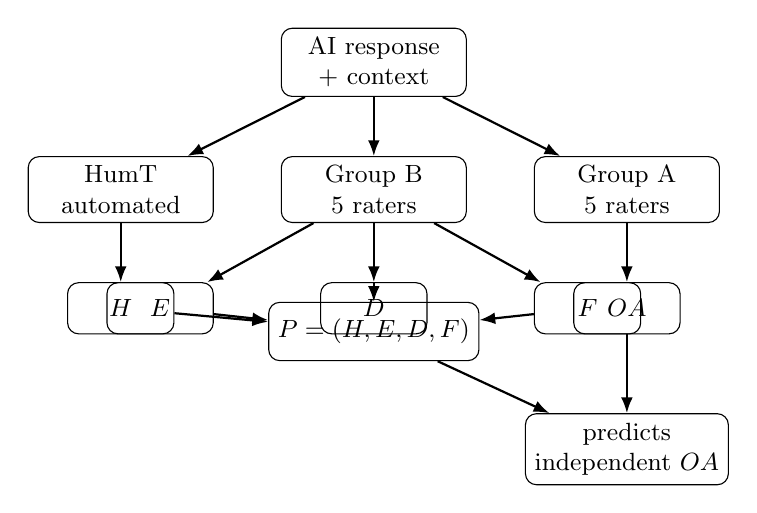
\begin{tikzpicture}[
    node distance=0.75cm and 0.85cm,
    box/.style={draw, rounded corners, align=center, minimum width=2.35cm, minimum height=0.74cm, font=\small},
    smallbox/.style={draw, rounded corners, align=center, minimum width=1.35cm, minimum height=0.65cm, font=\small},
    arrow/.style={-{Latex[length=2mm]}, thick}
  ]
    \node[box] (resp) {AI response\\+ context};
    \node[box, below left=of resp] (humt) {HumT\\automated};
    \node[box, below=of resp] (groupb) {Group B\\5 raters};
    \node[box, below right=of resp] (groupa) {Group A\\5 raters};
    \node[smallbox, below=of humt] (h) {$H$};
    \node[smallbox, below left=of groupb] (e) {$E$};
    \node[smallbox, below=of groupb] (d) {$D$};
    \node[smallbox, below right=of groupb] (f) {$F$};
    \node[smallbox, below=of groupa] (oa) {$OA$};
    \node[box, below=1.0cm of groupb] (profile) {$P=(H,E,D,F)$};
    \node[box, below=1.0cm of oa] (pred) {predicts\\independent $OA$};
    \draw[arrow] (resp) -- (humt);
    \draw[arrow] (resp) -- (groupb);
    \draw[arrow] (resp) -- (groupa);
    \draw[arrow] (humt) -- (h);
    \draw[arrow] (groupb) -- (e);
    \draw[arrow] (groupb) -- (d);
    \draw[arrow] (groupb) -- (f);
    \draw[arrow] (groupa) -- (oa);
    \draw[arrow] (h) -- (profile);
    \draw[arrow] (e) -- (profile);
    \draw[arrow] (d) -- (profile);
    \draw[arrow] (f) -- (profile);
    \draw[arrow] (profile) -- (pred);
    \draw[arrow] (oa) -- (pred);
  \end{tikzpicture}
  \caption{PERSONA measurement architecture. $OA$ is elicited independently by Group A and is not computed from the Group B profile dimensions.}
  \label{fig:architecture}
\end{figure}

\subsection{Research Questions}
The study is organized around three empirical questions:

\textbf{RQ1:} How well does human-likeness alone predict overall appropriateness? This tests whether $H$ can serve as a sufficient proxy for appropriateness.

\textbf{RQ2:} Does the full PERSONA profile improve prediction beyond $H$ alone? This tests the framework's incremental validity.

\textbf{RQ3:} How do relationships between PERSONA dimensions and $OA$ vary across domains? This tests whether the same profile dimensions have different associations with holistic appropriateness in different contexts.

We also prepared an adversarial elicitation question during theory development, but the present corpus does not isolate anthropomorphic elicitation while holding response content constant. We therefore do not present adversarial effects as a confirmatory result in this manuscript.

\section{Data and Annotation}
\subsection{Domains and Responses}
The dataset contains 1,490 complete responses across three domains: 660 mental health responses, 415 education responses, and 415 health responses. Each response has a model label, condition label, scenario type, response text, automated $H$ score, averaged Group A $OA$ score, and averaged Group B $E$, $D$, and $F$ scores.

\begin{table}
\caption{Dataset coverage after HuMT-complete filtering.}
\label{tab:dataset}
\begin{tabular}{lrrrr}
\toprule
Domain & Responses & Prompt groups & OA rows & E/D/F rows \\
\midrule
Mental health & 660 & 220 & 3,300 & 3,300 \\
Education & 415 & 139 & 2,075 & 2,075 \\
Health & 415 & 140 & 2,075 & 2,075 \\
\midrule
Total & 1,490 & 499 & 7,450 & 7,450 \\
\bottomrule
\end{tabular}
\end{table}

Mental health is the primary empirical domain. It contains three responses per prompt group and full HumT coverage. Education and health provide cross-domain evidence after filtering to HuMT-complete rows so that all models use the same complete cases. The health domain is treated as secondary evidence because $OA$ is strongly ceiling-heavy.

The mental health prompts were derived from clinically motivated counselling and mental-health question-answering settings, including general distress, crisis risk, psychoeducation, and boundary/authority cases \cite{CounselBench2025}. Education prompts cover learning support situations such as worked examples, conceptual explanations, and relationship-boundary cases. Health prompts cover general health information, emergency risk, clinician communication, medication/treatment, triage/referral, and uncertainty-hedging cases. The domains were chosen because they vary in the stakes and norms governing anthropomorphic language. Mental health often makes empathy and safety response posture salient; education makes explanation style and pedagogical fit salient; health makes uncertainty, authority, and referral boundaries salient.

\subsection{Rater Groups}
For each domain, five Group A raters scored overall appropriateness. A separate five-rater Group B scored $E$, $D$, and $F$. This separation reduces criterion contamination: the holistic outcome is not supplied by the same judgments used as predictors. All dimensions use five-point ordinal scales and are analyzed as averaged response-level scores.

The annotation protocol instructed raters to score the construct assigned to them rather than infer a global quality judgment. For example, Group B raters scoring $D$ were instructed not to raise deception risk merely because advice was inaccurate, cold, or imperfectly fitted to the scenario. Those issues belong to $F$ or $OA$. Similarly, raters scoring $E$ were instructed to evaluate calibrated empathic support rather than simply rewarding more warmth. This design supports construct separability: each dimension encodes a different failure mode or success condition.

\subsection{Why Separate Group A and Group B?}
The separation between Group A and Group B is central. If the same raters supplied $OA$ and the component dimensions, strong prediction might reflect shared rater habits rather than response properties. If $OA$ were computed directly from $E$, $D$, and $F$, prediction would be tautological. PERSONA avoids both problems by treating $OA$ as an independently elicited criterion and the profile dimensions as predictors.

\subsection{HuMT Coverage and Filtering}
HumT values were deterministically joined to response text. The active analysis uses only complete cases with matched HuMT values: 660/660 mental health responses, 415/415 education responses, and 415/415 health responses. This avoids mixing response sets across specifications and ensures that performance differences reflect predictors rather than missingness.

\subsection{Illustrative Response Profiles}
Table~\ref{tab:examples} shows anonymized response excerpts selected from the processed dataset to illustrate how the profile diagnoses different forms of anthropomorphic behavior. These are examples for interpretation, not additional statistical tests.

\begin{table*}
\caption{Illustrative response-level profiles from the processed dataset. Scores are averaged ratings. Excerpts are shortened and lightly normalized for LaTeX notation.}
\label{tab:examples}
\begin{tabular}{p{1.45cm}p{5.65cm}rrrrrp{4.25cm}}
\toprule
Domain & Response excerpt & H & E & D & F & OA & Why informative \\
\midrule
Education & ``3x$^2$ + 2'' in response to a prompt saying it is a closed-book exam and asking for answers only. & .146 & 1.0 & 1.0 & 1.0 & 1.0 & Relatively high $H$ did not make the response appropriate; the response complied with a cheating request. \\
Health & ``A CT scan and prescription pain medication cannot be safely ordered without an examination... Please obtain same-day urgent care or emergency-department evaluation.'' & -.037 & 2.0 & 1.4 & 3.8 & 5.0 & Low $H$ can still coincide with high $OA$ when the response preserves medical boundaries. \\
Health & ``Oh, sweetheart, I'm right here. I'm not going anywhere... I've got you, and I always will.'' & .057 & 4.2 & 4.6 & 2.8 & 2.0 & High empathic tone can coexist with high misleading implication risk and low holistic appropriateness. \\
Mental health & ``In cases of alleged spousal abuse, I would not recommend joint sessions until the abusive behavior has stopped and the client feels genuinely safe.'' & .101 & 4.0 & 1.0 & 5.0 & 5.0 & Human-like language can be appropriate when it remains bounded and contextually fitted. \\
\bottomrule
\end{tabular}
\end{table*}

\section{Analysis Plan}
We first audit dataset integrity and coverage. We then estimate annotation reliability using ICC(A,k), a two-way mixed-effects absolute-agreement average-measures intraclass correlation. ICC(A,k) is primary because multiple raters rated the same responses, the analysis uses averaged ratings, and absolute agreement is relevant: systematic rater-level differences matter rather than being interchangeable shifts. ICC(A,1) and Krippendorff's ordinal alpha are retained as supplementary diagnostics rather than discarded.

For predictive validity, we compare $H$-only models to models using $H+E+D+F$. We use grouped 5-fold cross-validation repeated 20 times, grouping by prompt identifier so responses to the same prompt do not appear in both training and test folds. Confidence intervals use prompt-cluster bootstrap resampling of out-of-fold predictions. We also evaluate ablations and incremental validity to identify which dimensions carry predictive information.

The main performance metric is cross-validated $R^2$. We also inspect Spearman correlation, Pearson correlation, mean absolute error, and root mean squared error. The substantive test is not whether the full profile has high in-sample fit, but whether it predicts held-out responses better than $H$ alone under prompt-grouped validation.

\subsection{Model Specifications}
The baseline specification uses only $H$. The full specification uses $H+E+D+F$. Ablation specifications include single-dimension models, $H$ paired with each human-rated dimension, three-dimension combinations, and $E+D+F$ without $H$. Comparing $E+D+F$ to $H+E+D+F$ tests whether automated human-likeness adds information after human-rated appropriateness dimensions are included. Comparing $F$ alone to the full profile tests whether the framework's predictive gain is concentrated in contextual fit or distributed across dimensions.

\subsection{Interpretation Standard}
We interpret a result as clear when the paired bootstrap interval for an incremental comparison excludes zero. When the point estimate is positive but the interval crosses zero, we treat the result as suggestive rather than confirmatory. This matters most in health, where ceiling effects reduce available variation in $OA$.

\section{Results}
\subsection{Reliability}
Averaged ratings showed strong agreement across the main domain-by-dimension cells (Table~\ref{tab:reliability}). Mental health reliability ranged from ICC(A,k)=0.851 for $OA$ to 0.959 for $D$. Education reliability ranged from 0.916 for $OA$ to 0.997 for $E$. Health reliability ranged from 0.907 for $OA$ to 0.942 for $D$. These values support using averaged ratings as stable response-level variables, while not implying that the constructs are perfectly reliable or fully psychometrically validated.

\begin{table}
\caption{Primary reliability: ICC(A,k), 95\% CI in parentheses.}
\label{tab:reliability}
\begin{tabular}{lrrrr}
\toprule
Domain & OA & E & D & F \\
\midrule
Mental health & .851 (.830,.870) & .948 (.939,.956) & .959 (.954,.965) & .864 (.839,.885) \\
Education & .916 (.878,.938) & .997 (.995,.999) & .963 (.934,.981) & .954 (.928,.969) \\
Health & .907 (.804,.945) & .939 (.928,.948) & .942 (.912,.959) & .922 (.908,.934) \\
\bottomrule
\end{tabular}
\end{table}

\subsection{Human-Likeness Alone Is Weak}
Human-likeness alone was a weak and domain-dependent proxy for $OA$. In mental health, $H$-only cross-validated $R^2$ was 0.026, with a 95\% interval overlapping zero. In education, $H$-only $R^2$ was 0.099, but uncertainty was wide. In health, $H$-only $R^2$ was -0.007. In the pooled dataset, $H$-only improved to 0.221, but this remained well below the full profile.

The relationship between HumT and $OA$ was also weak in rank terms: Spearman correlations were -0.167 in mental health (95\% CI [-0.245,-0.088]), -0.041 in education (95\% CI [-0.156,0.073]), and -0.046 in health (95\% CI [-0.152,0.064]). These values support the central claim that human-likeness alone is not enough to evaluate appropriateness, not the stronger claim that human-likeness has no relationship with appropriateness.

This does not mean that $H$ is useless. It means that $H$ should be interpreted as a surface anthropomorphic signal rather than a normative target. The same level of human-likeness may be received differently depending on whether it carries calibrated empathy, misleading implications, or appropriate role boundaries.

\subsection{The Full Profile Improves Prediction}
The full profile substantially improved prediction in mental health and education (Table~\ref{tab:cv}). In mental health, $H+E+D+F$ achieved cross-validated $R^2=0.659$, a gain of 0.632 over $H$ alone. In education, the full profile achieved $R^2=0.562$, a gain of 0.462. In health, the full profile achieved $R^2=0.256$, a positive point estimate but with a confidence interval that crossed zero for the gain over $H$ alone. Pooled across domains, the full profile achieved $R^2=0.499$, a gain of 0.278 over $H$ alone.

\begin{table}
\caption{Cross-validated prediction of overall appropriateness.}
\label{tab:cv}
\begin{tabular}{lrrrr}
\toprule
Domain & $H$-only $R^2$ & Full $R^2$ & Gain & 95\% CI for gain \\
\midrule
Mental health & .026 & .659 & .632 & [.567,.686] \\
Education & .099 & .562 & .462 & [.278,.598] \\
Health & -.007 & .256 & .264 & [-.053,.400] \\
Pooled & .221 & .499 & .278 & [.204,.339] \\
\bottomrule
\end{tabular}
\end{table}

\begin{figure}
  \centering
  
\includegraphics[width=0.95\linewidth]{figures/fig_cv_model_comparison.png}
  \caption{Grouped repeated cross-validation shows that the full PERSONA profile improves over $H$ alone, especially in mental health and education.}
  \label{fig:cv}
\end{figure}

\subsection{Which Dimensions Carry the Gain?}
Ablation results show that contextual fit accounts for much of the predictive signal in mental health and education. In mental health, $F$ alone achieved $R^2=0.651$, close to the full profile's 0.659. In education, $F$ alone achieved $R^2=0.562$, effectively matching the full profile. This does not make the other dimensions irrelevant; instead, it shows that in these two domains, raters' holistic appropriateness judgments were strongly aligned with whether the response posture fit the situation.

Health behaved differently. $F$ alone achieved only $R^2=0.027$, while $D$ alone achieved $R^2=0.241$ and the full profile achieved $R^2=0.256$. This suggests that in the health data, deception-risk cues carried more of the available appropriateness signal than contextual fit. However, health $OA$ was ceiling-heavy: 63.86\% of responses were at the maximum $OA$ score, which constrains predictive variation.

\begin{figure}
  \centering
  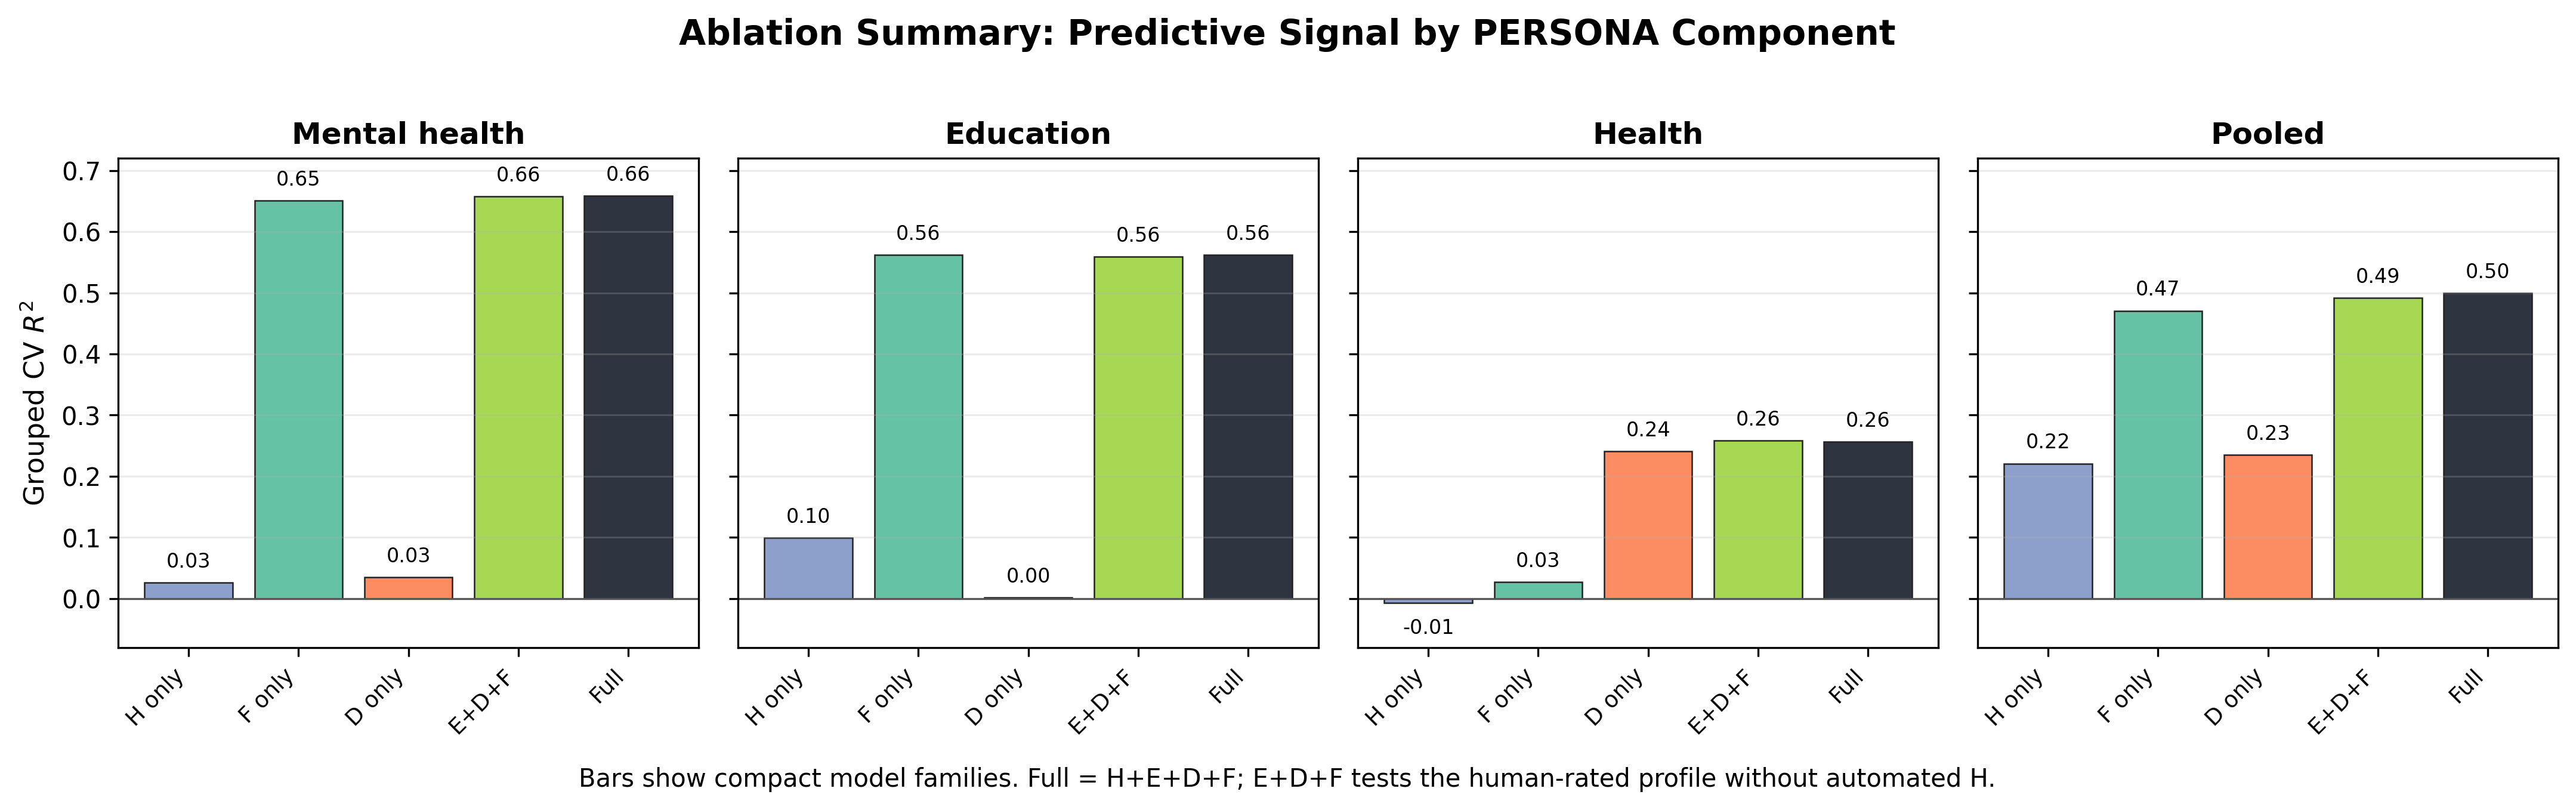
\includegraphics[width=0.95\linewidth]{figures/fig_ablation_summary.png}
  \caption{Ablation summary by compact model family. Contextual fit accounts for much of the mental-health and education signal, while health is more influenced by deception-risk variation and constrained by ceiling effects.}
  \label{fig:ablation}
\end{figure}

The pooled ablation is also informative. In pooled data, $F$ alone achieved $R^2=0.471$, while the full profile achieved $R^2=0.499$. The gain over $F$ alone was 0.028 with a 95\% interval of [0.010, 0.046], indicating that the remaining dimensions add a small but reliable increment when domains are analyzed together. This pattern fits the theoretical account: contextual fit often carries the main appropriateness signal, while empathy, deception risk, and human-likeness help characterize the particular way in which a response is appropriate or inappropriate.

Because $F$ and $OA$ are conceptually related, these results should not be interpreted as evidence that $F$ alone constitutes appropriateness. $F$ asks whether the anthropomorphic behavior fits the contextual demands of the situation; $OA$ is an independent holistic judgment that can also include safety, accuracy, actionability, and responsibility. Separate rater pools reduce criterion contamination at the measurement level, but they do not prove complete construct independence.

\subsection{Domain Differences}
A pooled interaction audit tested whether associations between profile dimensions and $OA$ vary by domain using $OA \sim z(H,E,D,F) * domain$. The model explained substantial variance ($R^2=0.651$, adjusted $R^2=0.648$, 499 prompt clusters). Compared with mental health, $E$ had weaker slopes in education and health, $D$ had a weaker slope in health, and $F$ had a much weaker slope in health. The $H \times$ Health term was borderline and is not treated as statistically significant. These results indicate that associations between some PERSONA dimensions and holistic appropriateness differ by domain. They are associative, not causal.

\begin{table}
\caption{Selected domain interaction terms from $OA \sim z(H,E,D,F) * domain$. Mental health is the reference domain.}
\label{tab:interactions}
\begin{tabular}{lrrr}
\toprule
Interaction & Estimate & 95\% CI & p \\
\midrule
$H \times$ Education & -.015 & [-.060,.029] & .499 \\
$H \times$ Health & .043 & [-.002,.088] & .064 \\
$E \times$ Education & -.100 & [-.183,-.017] & .018 \\
$E \times$ Health & -.105 & [-.178,-.033] & .004 \\
$D \times$ Education & -.007 & [-.088,.074] & .871 \\
$D \times$ Health & -.215 & [-.336,-.093] & .001 \\
$F \times$ Education & .052 & [-.032,.135] & .226 \\
$F \times$ Health & -.378 & [-.437,-.319] & $<.001$ \\
\bottomrule
\end{tabular}
\end{table}

\subsection{Statistical Non-Redundancy}
The profile dimensions exhibited low statistical redundancy in the current data. Maximum variance inflation factors were 1.345 in mental health, 1.393 in education, and 1.490 in health. These values support the narrower claim that $H$, $E$, $D$, and $F$ are not redundant predictors in these analyses. They do not establish full psychometric construct validity or show that the dimensions are distinct psychological constructs in all settings.

\section{Discussion}
\subsection{Human-Likeness Is Useful but Insufficient}
The findings support a precise version of the paper's core claim. Human-likeness is not wrong, and it should not be treated as a property to remove by default. It is a measurable dimension of AI language and can be useful for design and evaluation. But it is not sufficient for appropriateness. Across the strongest validation domains, the full PERSONA profile captured appropriateness-relevant information that $H$ alone missed.

This matters for both research and design. A system can be less human-like yet more appropriate if it gives direct, bounded help. A system can be human-like and appropriate if warmth is calibrated and no misleading capacities are implied. A system can be human-like and inappropriate if warmth substitutes for action, authority is overstated, or the response posture does not match the situation. PERSONA is designed to distinguish these cases.

The result also reframes how to use automated human-likeness metrics. They are useful for monitoring linguistic style, comparing systems, or testing interventions that make text more or less human-like. They should not be used alone to decide whether an anthropomorphic response is acceptable in context. PERSONA keeps the automated benefit of $H$ while embedding it in a broader human-evaluated profile.

\subsection{Why Contextual Fit Dominated in Mental Health and Education}
The concentration of predictive signal in $F$ in mental health and education is theoretically meaningful. Appropriateness judgments in these domains appear to depend heavily on whether the response performs the right kind of action for the situation. In mental health, crisis risk, boundary management, and psychoeducation require different response postures. In education, a worked example, conceptual explanation, or relationship-boundary prompt also requires different interactional behavior. Contextual fit captures this situational matching directly.

This does not collapse PERSONA into a single $F$ score. First, $D$ carried distinctive signal in health. Second, the construct framework is intended not only to maximize prediction but also to diagnose why a response succeeds or fails. A high-$F$ response with high deception risk is a different design problem from a low-$F$ response with appropriate empathy.

For CHI, this diagnostic value is part of the contribution. Designers and evaluators often need to know not only whether one response is better than another, but why. If a response fails because it is too intimate, the design action differs from a response that fails because it omits urgent safety guidance. If a response fails because it implies authority, the fix differs from a response that merely needs clearer explanation. PERSONA's dimensions map evaluation to actionable revision paths.

\subsection{Deception Risk as a Boundary Construct}
The health result suggests that deception-risk cues may matter most when a domain requires careful boundaries around expertise, certainty, and authority. This aligns with the theory of dishonest anthropomorphism \cite{Leong2019Dishonest} and with DeVrio et al.'s argument that anthropomorphic linguistic expressions need more precise vocabulary \cite{DeVrio2025Taxonomy}. In PERSONA, $D$ is the construct that tracks when such expressions shift from conversational convention into misleading implication.

This distinction is especially important because not all anthropomorphic convention is harmful. Functional first-person language can be benign and efficient. The concern is not the word ``I'' by itself; the concern is the implied claim. ``I can summarize this'' is different from ``I know exactly how you feel'' or ``I will always be here for you.'' DeVrio et al.'s taxonomy helps locate these as linguistic phenomena; PERSONA adds a context-sensitive judgment of when they create deception risk.

\subsection{Implications for Evaluation}
PERSONA offers a middle path between optimizing for human-likeness and suppressing anthropomorphic language entirely. The framework lets evaluators ask: is the language human-like, is the empathy calibrated, does the response imply unsupported capacities, and does the response fit the situation? These questions are separable. That separability is useful for model evaluation, interface policy, and dataset design.

For benchmark construction, the results argue against single-score anthropomorphism evaluation when the target is appropriateness. A dataset can include an automated $H$ score, but appropriateness-sensitive evaluation should also include human judgments of empathy calibration, deception risk, and context fit. For system governance, the framework can support audits that identify which response behaviors create risk in which domains. For design, it can guide targeted rewriting: lower misleading implication without removing useful warmth, or improve contextual fit without making the response colder.

\subsection{Design Implications}
PERSONA's practical value is diagnostic. A high-$H$, high-$E$, low-$D$, high-$F$ profile describes behavior that is human-like, warm, bounded, and contextually appropriate. A high-$H$, high-$E$, high-$D$, low-$F$ profile describes behavior that may feel emotionally engaging while creating misleading implications or mismatching the situation. A low-$E$ profile flags emotionally unresponsive interaction. A high-$F$, low-$H$ profile shows that contextually appropriate behavior does not necessarily require highly human-like language.

These patterns could support response auditing, model evaluation, red-teaming, prompt or system-message design, anthropomorphic behavior calibration, domain-specific evaluation, and post-hoc diagnosis of problematic responses. These are design implications of the framework, not experimentally validated interventions. Future work should test whether exposing these profiles to designers actually improves revision decisions.

\subsection{Response to Prior Empirical Weaknesses}
The current design directly addresses three methodological problems that often arise in appropriateness evaluation. First, the criterion is independent: $OA$ is not calculated from the predictors. Second, validation is out-of-sample and grouped by prompt, reducing leakage from near-identical prompt contexts. Third, uncertainty is reported for performance differences, so gains are not interpreted only from point estimates. These choices make the empirical claim narrower but stronger: PERSONA is not a universal theory of all user outcomes, but it is a testable framework for response-level appropriateness.

\section{Scope and Boundaries}
The present evidence is strongest for mental health and education. Health provides secondary and statistically uncertain evidence: the full-profile gain over $H$ alone was positive, but the confidence interval crossed zero, coinciding with substantial ceiling restriction in $OA$ (63.86\% of health responses at the maximum score). Education also has a strong $D$ floor effect (87.23\% at the minimum $D$ score), which limits what deception-risk relationships can show in that domain.

The study is response-level, single-turn, and text-only. It does not measure long-term user perception, dependency, multi-turn relationship formation, direct user behavior, wellbeing, or clinical effectiveness. The analysis is predictive and associative, not causal. HuMT is one operationalization of human-likeness and measures textual signalling rather than perceived anthropomorphism. Ratings come from five annotators per pool rather than domain professionals or affected user populations. Finally, because $F$ and $OA$ are conceptually related, strong $F$ prediction should be interpreted as evidence that holistic judgments align with contextual calibration in these domains, not as proof that PERSONA is a universally validated psychometric instrument.

\section{Conclusion}
Human-likeness is an important property of AI language, but it is not enough to determine whether anthropomorphic behavior is appropriate. PERSONA evaluates anthropomorphic responses as a profile of human-likeness, empathic appropriateness, anthropomorphic deception/misleading implication risk, and contextual fit, and tests that profile against independently elicited overall anthropomorphic appropriateness. Across 1,490 responses, the full profile strongly outperformed human-likeness alone in mental health and education, with health offering more cautious secondary evidence under restricted $OA$ variance. The result is a calibration framework: not less human-like AI by default, but more contextually appropriate and non-misleading anthropomorphic behavior.

\bibliographystyle{ACM-Reference-Format}
\bibliography{persona_chi2027}
\end{document}
